\section{变换}\label{sec:变换}

通常,\keyindex{变换}{transformation}{}$\bm T$是
从点到点和从向量到向量的映射:
\begin{align*}
    \bm p'=\bm T(\bm p), \  \bm v'=\bm T(\bm v)\, .
\end{align*}

变换$\bm T$可以是任意过程。
然而,本章我们考虑所有可能变换的一个子集。
特别地,它们是:
\begin{itemize}
    \item \keyindex{线性的}{linear}{}:对于任意线性变换$\bm T$和
          标量$s$,都有$\bm T(s\bm v)=s\bm T(\bm v)$以及
          $\bm T(\bm v_1+\bm v_2)=\bm T(\bm v_1)+\bm T(\bm v_2)$。
          这两点性质可极大简化关于变换的推导。
    \item \keyindex{连续的}{continuous}{}:简单说,
          $\bm T$把$\bm p$和$\bm v$的邻域映射为$\bm p'$和$\bm v'$的邻域。
    \item \keyindex{一对一}{one-to-one}{}且\keyindex{可逆}{invertible}{}:
          对于每个$\bm p$,$\bm T$把$\bm p$映射为唯一一个$\bm p'$。
          此外,存在一个逆变换$\bm T^{-1}$将$\bm p'$映射回$\bm p$。
\end{itemize}

我们经常想取某一坐标系下的点、向量或法线并求它在另一坐标系下的坐标值。
运用线性代数的基本性质,可以证明一个$4\times4$的矩阵
能表示点或向量从一个坐标系到另一个坐标系的线性变换。
此外,这样的$4\times4$矩阵足以表达固定坐标系内点和向量的所有线性变换,
例如空间中平移或绕一点旋转。
因此,有两种不同(且不兼容!)的方式解释矩阵:
\begin{itemize}
    \item \keyindex{坐标系的变换}{transformation of the frame}{}:给定一点,
          矩阵可表示如何计算同一坐标系下的\emph{新}点来代表对原始点的变换
          (例如朝某个方向平移)。
    \item \keyindex{从一个坐标系到另一个的变换}{transformation from one frame to another}{}:
          矩阵可依据一点或向量在原坐标系的坐标来表示其在新坐标系的坐标。
\end{itemize}

pbrt中所用的变换大多数是点从一个坐标系到另一个坐标系的变换。

通常,变换使得在最方便的坐标空间内工作成为可能。
例如,我们编写定义虚拟相机的例程,
假设相机位于原点,看向$z$轴,且$y$向上,$x$轴向右。
这些假设极大简化了相机实现。
然后,为了把相机置于场景中任意一点并看向任意方向,
我们只需要构造一个变换把场景坐标系统中的点映射到相机坐标系统中
(关于pbrt中相机坐标空间的更多信息详见\refsub{相机坐标空间})。

\subsection{齐次坐标}\label{sub:齐次坐标}
给定由$(\bm p_\mathrm{o},\bm v_1,\bm v_2,\bm v_3)$定义的坐标系,
具有相同坐标$(x,y,z)$的点$(p_x,p_y,p_z)$和向量$(v_x,v_y,v_z)$在表示上有歧义。
利用本章开头介绍的点和向量的表示,
我们可以把点写作内积$[s_1\ s_2\ s_3\ 1][\bm v_1\ \bm v_2\ \bm v_3\ \bm p_\mathrm{o}]^\mathrm{T}$,
把向量写作内积$[s'_1\ s'_2\ s'_3\ 0][\bm v_1\ \bm v_2\ \bm v_3\ \bm p_\mathrm{o}]^\mathrm{T}$。
这样有三个$s_i$以及一个零或一的四维向量称作点或向量的\keyindex{齐次}{homogeneous}{}表示。
齐次表示的第四个坐标有时称作\keyindex{权重}{weight}{}。
对于一个点,它的值可以是任意非零标量:
齐次点$[1,3,-2,1]$和$[-2,-6,4,-2]$描述了同一个笛卡尔点$(1,3,-2)$。
把齐次点转换为普通点需要用前三个分量除以权重
\sidenote{译者注:这里调整了原文对各种括号的混用。
    齐次坐标和矩阵等用方括号,一般坐标等用圆括号。}:
\begin{align*}
    [x,y,z,w]\rightarrow\left(\frac{x}{w},\frac{y}{w},\frac{z}{w}\right)\, .
\end{align*}

我们将利用这些事实来看看变换矩阵为什么可以描述
如何将一个坐标系下的点和向量映射到另一个坐标系。
考虑矩阵$\bm M$描述从一个坐标系到另一个坐标系的变换:
\begin{align*}
    M=\left[
        \begin{array}{cccc}
            m_{0,0} & m_{0,1} & m_{0,2} & m_{0,3} \\
            m_{1,0} & m_{1,1} & m_{1,2} & m_{1,3} \\
            m_{2,0} & m_{2,1} & m_{2,2} & m_{2,3} \\
            m_{3,0} & m_{3,1} & m_{3,2} & m_{3,3}
        \end{array}
        \right]\, .
\end{align*}

(本书中,我们定义矩阵元素时索引从零开始,这样公式和源码更能直接对应。)
若$\bm M$表示的变换被应用到$x$轴向量$(1,0,0)$上,我们有
\begin{align*}
    \bm M\bm x=\bm M[1\ 0\ 0\ 0]^\mathrm{T}=[m_{0,0}\ m_{1,0}\ m_{2,0}\ m_{3,0}]^\mathrm{T}\, .
\end{align*}

因此,直接阅读矩阵的列就能知道当前坐标系统的基向量和原点是怎样被矩阵变换的:
\begin{align*}
    \bm M\bm y & =[m_{0,1}\ m_{1,1}\ m_{2,1}\ m_{3,1}]^\mathrm{T}\, , \\
    \bm M\bm z & =[m_{0,2}\ m_{1,2}\ m_{2,2}\ m_{3,2}]^\mathrm{T}\, , \\
    \bm M\bm p & =[m_{0,3}\ m_{1,3}\ m_{2,3}\ m_{3,3}]^\mathrm{T}\, .
\end{align*}

一般通过表征基是如何变换的,
我们就能知道该基表示的任意指定点或向量是如何被变换的。
因为当前坐标系统的点和向量由当前坐标系表示,
直接对它们施加变换等价于对当前坐标系统的基施加变换并
用变换后的基求出坐标。

我们并不在代码中显式地使用齐次坐标;
pbrt中没有类{\ttfamily Homogeneous}。
然而,下节各种变换例程都隐式地将点、向量和法线转换为齐次形式,
变换齐次点,再转换回来返回结果。
这样就在一个地方(即变换的实现)隔离了齐次坐标的细节。
\begin{lstlisting}
`\initcode{Transform Declarations}{=}`
class `\initvar{Transform}{}` {
public:
    `\refcode{Transform Public Methods}{}`
private:
    `\refcode{Transform Private Data}{}`
};
\end{lstlisting}

变换由矩阵\refvar[Transform::m]{m}{},即一个\refvar{Matrix4x4}{}对象的元素表示。
底层类\refvar{Matrix4x4}{}定义在\refsub{4x4矩阵}。
矩阵\refvar[Transform::m]{m}{}按\keyindex{行优先}{row-major}{}形式存储,
所以元素{\ttfamily m[i][j]}对应$m_{i,j}$,
其中$i$是行数,$j$是列数。
为了方便,\refvar{Transform}{}还存储了
矩阵\refvar[Transform::m]{m}{}的逆
\refvar{Transform::mInv}{}成员;
因为pbrt的需要,易获取的逆比按需重复计算更好。

变换的这种表示相对更耗内存:
假设存储一个\refvar{Float}{}值需要4字节,一个
\refvar{Transform}{}就需要128字节存储。
幼稚地使用该方法会造成浪费;
如果一个场景有几百万个形状但仅有几千个不同的变换,
就更没理由在内存中冗余地多次保存同一个变换。
因此pbrt中的\refvar{Shape}{}保存的是\refvar{Transform}{}的指针,
\refsub{形状}定义的场景指定代码使用\refvar{TransformCache}{}来保证
所有共享同一变换的形状指向内存中该变换的单一实例。

这个共享变换的决定意味着丧失了灵活性,然而:
如果\refvar{Transform}{}被场景中的多个物体(以及不希望它改变的对象)共享,
则\refvar{Transform}{}的元素在创建后不能被修改。
现实中这点限制不是问题,
因为场景中的变换通常是在pbrt解析场景描述文件时创建的,
之后在渲染时不需要改变。
\begin{lstlisting}
`\initcode{Transform Private Data}{=}`
`\refvar{Matrix4x4}{}` `\initvar[Transform::m]{m}{}`, `\initvar[Transform::mInv]{mInv}{}`;
\end{lstlisting}

\subsection{基本运算}\label{sub:基本运算}
当创建新的\refvar{Transform}{}时,
它默认为\keyindex{恒等变换}{identity transformation}{transformation变换}——
将每个点和向量映射为它自己的变换。
该变换由\keyindex{单位矩阵}{identity matrix}{}表示:
\begin{align*}
    \bm I=\left[
        \begin{array}{cccc}
            1 & 0 & 0 & 0 \\
            0 & 1 & 0 & 0 \\
            0 & 0 & 1 & 0 \\
            0 & 0 & 0 & 1
        \end{array}
        \right]\, .
\end{align*}

这里的实现依赖\refvar{Matrix4x4}{}默认构造函数
把\refvar[Transform::m]{m}{}和\refvar[Transform::mInv]{mInv}{}填充为单位矩阵。
\begin{lstlisting}
`\initcode{Transform Public Methods}{=}\initnext{TransformPublicMethods}`
`\refvar{Transform}{}`() { }
\end{lstlisting}

\refvar{Transform}{}也可以从给定矩阵创建。
这时,给定矩阵必须是显式可逆的。
\begin{lstlisting}
`\refcode{Transform Public Methods}{+=}\lastnext{TransformPublicMethods}`
`\refvar{Transform}{}`(const `\refvar{Float}{}` mat[4][4]) {
    `\refvar[Transform::m]{m}{}` = `\refvar{Matrix4x4}{}`(mat[0][0], mat[0][1], mat[0][2], mat[0][3],
                  mat[1][0], mat[1][1], mat[1][2], mat[1][3],
                  mat[2][0], mat[2][1], mat[2][2], mat[2][3],
                  mat[3][0], mat[3][1], mat[3][2], mat[3][3]);
    `\refvar[Transform::mInv]{mInv}{}` = `\refvar[Matrix4x4::Inverse]{Inverse}{}`(`\refvar[Transform::m]{m}{}`);
}
\end{lstlisting}

\begin{lstlisting}
`\refcode{Transform Public Methods}{+=}\lastnext{TransformPublicMethods}`
`\refvar{Transform}{}`(const `\refvar{Matrix4x4}{}` &m) : `\refvar[Transform::m]{m}{}`(m), `\refvar[Transform::mInv]{mInv}{}`(`\refvar[Matrix4x4::Inverse]{Inverse}{}`(m)) { }
\end{lstlisting}

最常用的构造函数取变换矩阵的引用以及显式提供的逆。
在构造函数中计算逆是一种很好的方法,
因为许多几何变换有很简单的逆,
我们可以避免由于计算一般$4\times4$矩阵的逆
而造成的开销和潜在的数值精度损失。
\begin{lstlisting}
`\refcode{Transform Public Methods}{+=}\lastnext{TransformPublicMethods}`
`\refvar{Transform}{}`(const `\refvar{Matrix4x4}{}` &m, const `\refvar{Matrix4x4}{}` &mInv) 
   : `\refvar[Transform::m]{m}{}`(m), `\refvar[Transform::mInv]{mInv}{}`(mInv) {
}
\end{lstlisting}

\refvar{Transform}{}表示\refvar{Transform}{}的逆只需
通过交换\refvar[Transform::mInv]{mInv}{}和\refvar[Transform::m]{m}{}并返回。
\begin{lstlisting}
`\refcode{Transform Public Methods}{+=}\lastnext{TransformPublicMethods}`
friend `\refvar{Transform}{}` `\initvar[Transform::Inverse]{Inverse}{}`(const `\refvar{Transform}{}` &t) {
    return `\refvar{Transform}{}`(t.`\refvar[Transform::mInv]{mInv}{}`, t.`\refvar[Transform::m]{m}{}`);
}
\end{lstlisting}

转置变换中的两个矩阵以计算新变换也很有用。
\begin{lstlisting}
`\refcode{Transform Public Methods}{+=}\lastnext{TransformPublicMethods}`
friend `\refvar{Transform}{}` `\initvar[Transform::Transpose]{Transpose}{}`(const `\refvar{Transform}{}` &t) {
    return `\refvar{Transform}{}`(`\refvar[Matrix4x4::Transpose]{Transpose}{}`(t.`\refvar[Transform::m]{m}{}`), `\refvar[Matrix4x4::Transpose]{Transpose}{}`(t.`\refvar[Transform::mInv]{mInv}{}`));
}
\end{lstlisting}

我们提供了\refvar{Transform}{}相等(和不相等)测试方法;
它们的实现很简单就不介绍了\sidenote{译者注:即逐元素比较。}。
\refvar{Transform}{}也提供了方法{\ttfamily IsIdentity()}检查变换是否是恒等的。

\subsection{平移}\label{sub:平移}
最简单的变换之一就是\keyindex{平移变换}{translation transformation}{transformation变换},
$\bm T(\Delta x,\Delta y, \Delta z)$。
当施加到一点$\bm p$上时,它将$\bm p$的坐标平移$\Delta x,\Delta y$和$\Delta z$,
如\reffig{2.10}所示。例如,
\begin{figure}[htbp]
    \centering%LaTeX with PSTricks extensions
%%Creator: Inkscape 1.0.1 (3bc2e813f5, 2020-09-07)
%%Please note this file requires PSTricks extensions
\psset{xunit=.5pt,yunit=.5pt,runit=.5pt}
\begin{pspicture}(200.08000183,227.47000122)
{
\newrgbcolor{curcolor}{0 0 0}
\pscustom[linewidth=1,linecolor=curcolor]
{
\newpath
\moveto(5.5,160.20000122)
\lineto(5.5,6.16000122)
\lineto(160.1,6.16000122)
}
}
{
\newrgbcolor{curcolor}{0 0 0}
\pscustom[linestyle=none,fillstyle=solid,fillcolor=curcolor]
{
\newpath
\moveto(0,155.29000122)
\lineto(5.5,159.55000122)
\lineto(11.01,155.29000122)
\lineto(5.5,168.30000122)
\closepath
}
}
{
\newrgbcolor{curcolor}{0.65098041 0.65098041 0.65098041}
\pscustom[linestyle=none,fillstyle=solid,fillcolor=curcolor]
{
\newpath
\moveto(1.2,156.84000122)
\lineto(5.5,166.99000122)
\lineto(5.5,160.18000122)
\closepath
}
}
{
\newrgbcolor{curcolor}{0.40000001 0.40000001 0.40000001}
\pscustom[linestyle=none,fillstyle=solid,fillcolor=curcolor]
{
\newpath
\moveto(9.8,156.84000122)
\lineto(5.5,166.99000122)
\lineto(5.5,160.18000122)
\closepath
}
}
{
\newrgbcolor{curcolor}{0 0 0}
\pscustom[linestyle=none,fillstyle=solid,fillcolor=curcolor]
{
\newpath
\moveto(155.19,0.66000122)
\lineto(159.45,6.16000122)
\lineto(155.19,11.67000122)
\lineto(168.21,6.16000122)
\closepath
}
}
{
\newrgbcolor{curcolor}{0.65098041 0.65098041 0.65098041}
\pscustom[linestyle=none,fillstyle=solid,fillcolor=curcolor]
{
\newpath
\moveto(156.75,1.86000122)
\lineto(166.89,6.16000122)
\lineto(160.08,6.16000122)
\closepath
}
}
{
\newrgbcolor{curcolor}{0.40000001 0.40000001 0.40000001}
\pscustom[linestyle=none,fillstyle=solid,fillcolor=curcolor]
{
\newpath
\moveto(156.75,10.46000122)
\lineto(166.89,6.16000122)
\lineto(160.08,6.16000122)
\closepath
}
}
{
\newrgbcolor{curcolor}{0 0 0}
\pscustom[linestyle=none,fillstyle=solid,fillcolor=curcolor]
{
\newpath
\moveto(84.42999887,79.00999451)
\curveto(84.42999887,84.55180789)(77.73019729,87.32615393)(73.81201848,83.40797512)
\curveto(69.89383966,79.4897963)(72.6681857,72.78999472)(78.20999908,72.78999472)
\curveto(83.75181247,72.78999472)(86.52615851,79.4897963)(82.60797969,83.40797512)
\curveto(78.68980087,87.32615393)(71.98999929,84.55180789)(71.98999929,79.00999451)
\curveto(71.98999929,73.46818112)(78.68980087,70.69383508)(82.60797969,74.6120139)
\curveto(86.52615851,78.53019272)(83.75181247,85.2299943)(78.20999908,85.2299943)
\curveto(72.6681857,85.2299943)(69.89383966,78.53019272)(73.81201848,74.6120139)
\curveto(77.73019729,70.69383508)(84.42999887,73.46818112)(84.42999887,79.00999451)
\closepath
}
}
{
\newrgbcolor{curcolor}{0 0 0}
\pscustom[linewidth=1,linecolor=curcolor,linestyle=dashed,dash=4]
{
\newpath
\moveto(78.21,79.01000122)
\lineto(166.54,79.01000122)
\lineto(166.54,214.43000122)
}
}
{
\newrgbcolor{curcolor}{0 0 0}
\pscustom[linestyle=none,fillstyle=solid,fillcolor=curcolor]
{
\newpath
\moveto(173.05999613,212.30000114)
\curveto(173.05999613,217.84181453)(166.36019455,220.61616057)(162.44201573,216.69798175)
\curveto(158.52383691,212.77980293)(161.29818296,206.08000135)(166.83999634,206.08000135)
\curveto(172.38180972,206.08000135)(175.15615576,212.77980293)(171.23797695,216.69798175)
\curveto(167.31979813,220.61616057)(160.61999655,217.84181453)(160.61999655,212.30000114)
\curveto(160.61999655,206.75818776)(167.31979813,203.98384172)(171.23797695,207.90202054)
\curveto(175.15615576,211.82019935)(172.38180972,218.52000093)(166.83999634,218.52000093)
\curveto(161.29818296,218.52000093)(158.52383691,211.82019935)(162.44201573,207.90202054)
\curveto(166.36019455,203.98384172)(173.05999613,206.75818776)(173.05999613,212.30000114)
\closepath
}
}
{
\newrgbcolor{curcolor}{0 0 0}
\pscustom[linestyle=none,fillstyle=solid,fillcolor=curcolor]
{
\newpath
\moveto(72.01400587,53.52381757)
\curveto(71.94561637,53.21606481)(71.91142162,53.18187006)(71.87722687,53.14767531)
\curveto(71.77464261,53.11348056)(71.53527935,53.11348056)(71.33011084,53.11348056)
\curveto(70.95396857,53.11348056)(70.54363156,53.11348056)(70.54363156,52.49797503)
\curveto(70.54363156,52.25861177)(70.74880006,52.08763801)(70.98816333,52.08763801)
\curveto(71.60366885,52.08763801)(72.32175864,52.15602751)(72.97145892,52.15602751)
\curveto(73.7579382,52.15602751)(74.57861224,52.08763801)(75.33089677,52.08763801)
\curveto(75.46767578,52.08763801)(75.8780128,52.08763801)(75.8780128,52.73733829)
\curveto(75.8780128,53.11348056)(75.53606528,53.11348056)(75.33089677,53.11348056)
\curveto(75.02314401,53.11348056)(74.64700174,53.11348056)(74.37344373,53.14767531)
\lineto(75.33089677,56.94329273)
\curveto(75.63864954,56.63553997)(76.35673932,56.15681344)(77.51936087,56.15681344)
\curveto(81.3149783,56.15681344)(83.67441616,59.61048335)(83.67441616,62.58542674)
\curveto(83.67441616,65.28681211)(81.65692581,66.17587565)(79.84460398,66.17587565)
\curveto(78.30584016,66.17587565)(77.17741336,65.32100686)(76.83546584,65.0132541)
\curveto(75.98059705,66.17587565)(74.54441749,66.17587565)(74.30505423,66.17587565)
\curveto(73.51857494,66.17587565)(72.86887466,65.73134388)(72.42434289,64.9448646)
\curveto(71.87722687,64.05580106)(71.5694741,62.8931795)(71.5694741,62.79059525)
\curveto(71.5694741,62.48284248)(71.91142162,62.48284248)(72.11659013,62.48284248)
\curveto(72.35595339,62.48284248)(72.42434289,62.48284248)(72.52692715,62.58542674)
\curveto(72.59531665,62.61962149)(72.59531665,62.68801099)(72.73209566,63.23512702)
\curveto(73.14243267,64.97905935)(73.65535395,65.38939637)(74.20246997,65.38939637)
\curveto(74.44183323,65.38939637)(74.71539125,65.32100686)(74.71539125,64.60291708)
\curveto(74.71539125,64.26096956)(74.64700174,63.9532168)(74.57861224,63.64546404)
\closepath
\moveto(77.04063435,63.98741155)
\curveto(77.65613988,64.73969609)(78.68198243,65.38939637)(79.74201973,65.38939637)
\curveto(81.10980979,65.38939637)(81.21239404,64.22677481)(81.21239404,63.74804829)
\curveto(81.21239404,62.61962149)(80.46010951,59.91823612)(80.11816199,59.06336733)
\curveto(79.43426696,57.49040876)(78.37422966,56.94329273)(77.48516612,56.94329273)
\curveto(76.18576556,56.94329273)(75.67284429,57.96913528)(75.67284429,58.20849854)
\lineto(75.70703904,58.5162513)
\closepath
\moveto(77.04063435,63.98741155)
}
}
{
\newrgbcolor{curcolor}{0 0 0}
\pscustom[linestyle=none,fillstyle=solid,fillcolor=curcolor]
{
\newpath
\moveto(176.98786387,203.48647417)
\curveto(176.91947437,203.17872141)(176.88527962,203.14452666)(176.85108487,203.11033191)
\curveto(176.74850061,203.07613716)(176.50913735,203.07613716)(176.30396884,203.07613716)
\curveto(175.92782657,203.07613716)(175.51748956,203.07613716)(175.51748956,202.46063163)
\curveto(175.51748956,202.22126837)(175.72265806,202.05029461)(175.96202133,202.05029461)
\curveto(176.57752685,202.05029461)(177.29561664,202.11868411)(177.94531692,202.11868411)
\curveto(178.7317962,202.11868411)(179.55247024,202.05029461)(180.30475477,202.05029461)
\curveto(180.44153378,202.05029461)(180.8518708,202.05029461)(180.8518708,202.69999489)
\curveto(180.8518708,203.07613716)(180.50992328,203.07613716)(180.30475477,203.07613716)
\curveto(179.99700201,203.07613716)(179.62085974,203.07613716)(179.34730173,203.11033191)
\lineto(180.30475477,206.90594933)
\curveto(180.61250754,206.59819657)(181.33059732,206.11947004)(182.49321887,206.11947004)
\curveto(186.2888363,206.11947004)(188.64827416,209.57313995)(188.64827416,212.54808334)
\curveto(188.64827416,215.24946871)(186.63078381,216.13853225)(184.81846198,216.13853225)
\curveto(183.27969816,216.13853225)(182.15127136,215.28366346)(181.80932384,214.9759107)
\curveto(180.95445505,216.13853225)(179.51827549,216.13853225)(179.27891223,216.13853225)
\curveto(178.49243294,216.13853225)(177.84273266,215.69400048)(177.39820089,214.9075212)
\curveto(176.85108487,214.01845766)(176.5433321,212.8558361)(176.5433321,212.75325185)
\curveto(176.5433321,212.44549908)(176.88527962,212.44549908)(177.09044813,212.44549908)
\curveto(177.32981139,212.44549908)(177.39820089,212.44549908)(177.50078515,212.54808334)
\curveto(177.56917465,212.58227809)(177.56917465,212.65066759)(177.70595366,213.19778362)
\curveto(178.11629067,214.94171595)(178.62921195,215.35205297)(179.17632797,215.35205297)
\curveto(179.41569123,215.35205297)(179.68924925,215.28366346)(179.68924925,214.56557368)
\curveto(179.68924925,214.22362616)(179.62085974,213.9158734)(179.55247024,213.60812064)
\closepath
\moveto(182.01449235,213.95006815)
\curveto(182.62999788,214.70235269)(183.65584043,215.35205297)(184.71587773,215.35205297)
\curveto(186.08366779,215.35205297)(186.18625204,214.18943141)(186.18625204,213.71070489)
\curveto(186.18625204,212.58227809)(185.43396751,209.88089272)(185.09201999,209.02602393)
\curveto(184.40812496,207.45306536)(183.34808766,206.90594933)(182.45902412,206.90594933)
\curveto(181.15962356,206.90594933)(180.64670229,207.93179188)(180.64670229,208.17115514)
\lineto(180.68089704,208.4789079)
\closepath
\moveto(182.01449235,213.95006815)
}
}
{
\newrgbcolor{curcolor}{0 0 0}
\pscustom[linestyle=none,fillstyle=solid,fillcolor=curcolor]
{
\newpath
\moveto(193.37289352,222.50887422)
\curveto(193.50967253,222.74823748)(193.50967253,222.88501648)(193.50967253,222.98760074)
\curveto(193.50967253,223.46632726)(193.09933551,223.80827478)(192.62060899,223.80827478)
\curveto(192.03929821,223.80827478)(191.86832445,223.32954825)(191.79993495,223.09018499)
\lineto(189.78244461,216.49059794)
\curveto(189.74824986,216.45640319)(189.67986035,216.28542943)(189.67986035,216.25123468)
\curveto(189.67986035,216.08026092)(190.15858687,215.90928717)(190.29536588,215.90928717)
\curveto(190.39795013,215.90928717)(190.39795013,215.94348192)(190.50053439,216.18284518)
\closepath
\moveto(193.37289352,222.50887422)
}
}
{
\newrgbcolor{curcolor}{0 0 0}
\pscustom[linestyle=none,fillstyle=solid,fillcolor=curcolor]
{
\newpath
\moveto(178.80189615,9.25652985)
\curveto(178.93867516,9.80364588)(179.45159643,11.82113622)(180.9561655,11.82113622)
\curveto(181.05874976,11.82113622)(181.60586578,11.82113622)(182.05039755,11.54757821)
\curveto(181.43489202,11.4107992)(181.02455501,10.89787793)(181.02455501,10.3507619)
\curveto(181.02455501,10.00881439)(181.26391827,9.59847737)(181.84522904,9.59847737)
\curveto(182.32395556,9.59847737)(183.0078506,9.97461964)(183.0078506,10.86368318)
\curveto(183.0078506,11.99210998)(181.74264479,12.29986274)(180.99036025,12.29986274)
\curveto(179.72515445,12.29986274)(178.97286991,11.13724119)(178.6993119,10.65851467)
\curveto(178.15219587,12.09469423)(176.98957432,12.29986274)(176.33987404,12.29986274)
\curveto(174.08302044,12.29986274)(172.81781463,9.49589311)(172.81781463,8.94877709)
\curveto(172.81781463,8.70941383)(173.05717789,8.70941383)(173.09137264,8.70941383)
\curveto(173.2623464,8.70941383)(173.3307359,8.77780333)(173.36493066,8.94877709)
\curveto(174.11721519,11.2740202)(175.55339476,11.82113622)(176.30567929,11.82113622)
\curveto(176.71601631,11.82113622)(177.46830084,11.61596771)(177.46830084,10.3507619)
\curveto(177.46830084,9.66686687)(177.09215858,8.23068731)(176.30567929,5.15315967)
\curveto(175.96373177,3.81956436)(175.17725249,2.89630606)(174.21979944,2.89630606)
\curveto(174.08302044,2.89630606)(173.60429392,2.89630606)(173.12556739,3.16986408)
\curveto(173.67268342,3.30664308)(174.15140994,3.75117485)(174.15140994,4.36668038)
\curveto(174.15140994,4.94799116)(173.67268342,5.11896491)(173.36493066,5.11896491)
\curveto(172.68103562,5.11896491)(172.16811435,4.57184889)(172.16811435,3.85375911)
\curveto(172.16811435,2.86211131)(173.22815165,2.41757954)(174.18560469,2.41757954)
\curveto(175.65597901,2.41757954)(176.4424583,3.95634336)(176.47665305,4.05892762)
\curveto(176.75021106,3.27244833)(177.53669035,2.41757954)(178.83609091,2.41757954)
\curveto(181.09294451,2.41757954)(182.32395556,5.22154917)(182.32395556,5.76866519)
\curveto(182.32395556,6.00802846)(182.15298181,6.00802846)(182.0845923,6.00802846)
\curveto(181.87942379,6.00802846)(181.84522904,5.9054442)(181.77683954,5.76866519)
\curveto(181.05874976,3.40922734)(179.58837544,2.89630606)(178.90448041,2.89630606)
\curveto(178.04961162,2.89630606)(177.7076641,3.58020109)(177.7076641,4.33248563)
\curveto(177.7076641,4.81121215)(177.81024836,5.28993867)(178.04961162,6.24739172)
\closepath
\moveto(178.80189615,9.25652985)
}
}
{
\newrgbcolor{curcolor}{0 0 0}
\pscustom[linestyle=none,fillstyle=solid,fillcolor=curcolor]
{
\newpath
\moveto(11.63492206,186.97506843)
\curveto(11.73750631,187.2828212)(11.73750631,187.31701595)(11.73750631,187.48798971)
\curveto(11.73750631,187.86413197)(11.42975355,188.06930048)(11.08780603,188.06930048)
\curveto(10.88263752,188.06930048)(10.54069001,187.93252148)(10.3355215,187.62476871)
\curveto(10.30132674,187.48798971)(10.09615824,186.83828943)(10.02776873,186.42795241)
\curveto(9.85679497,185.88083638)(9.72001597,185.26533085)(9.58323696,184.68402008)
\lineto(8.59158917,180.75162365)
\curveto(8.52319966,180.44387088)(7.56574662,178.90510706)(6.12956705,178.90510706)
\curveto(5.035335,178.90510706)(4.79597174,179.86256011)(4.79597174,180.68323414)
\curveto(4.79597174,181.67488194)(5.17211401,183.042672)(5.89020379,184.95757809)
\curveto(6.23215131,185.84664163)(6.33473556,186.08600489)(6.33473556,186.53053666)
\curveto(6.33473556,187.48798971)(5.65084053,188.30866374)(4.55660848,188.30866374)
\curveto(2.47072864,188.30866374)(1.68424935,185.12855185)(1.68424935,184.95757809)
\curveto(1.68424935,184.71821483)(1.88941786,184.71821483)(1.92361261,184.71821483)
\curveto(2.16297587,184.71821483)(2.16297587,184.78660433)(2.26556013,185.12855185)
\curveto(2.88106566,187.18023694)(3.73593444,187.82993722)(4.48821898,187.82993722)
\curveto(4.65919274,187.82993722)(5.035335,187.82993722)(5.035335,187.14604219)
\curveto(5.035335,186.59892616)(4.79597174,186.01761539)(4.65919274,185.60727837)
\curveto(3.7701292,183.28203526)(3.39398693,182.05102421)(3.39398693,181.02518166)
\curveto(3.39398693,179.07608082)(4.76177699,178.42638054)(6.06117755,178.42638054)
\curveto(6.91604634,178.42638054)(7.63413612,178.80252281)(8.24964165,179.41802834)
\curveto(7.97608364,178.28960154)(7.70252563,177.19536949)(6.84765684,176.03274793)
\curveto(6.26634606,175.31465815)(5.44567202,174.66495787)(4.45402423,174.66495787)
\curveto(4.14627146,174.66495787)(3.15462367,174.73334737)(2.7784814,175.58821616)
\curveto(3.12042892,175.58821616)(3.42818168,175.58821616)(3.70173969,175.86177417)
\curveto(3.94110295,176.03274793)(4.14627146,176.3405007)(4.14627146,176.75083771)
\curveto(4.14627146,177.43473275)(3.56496069,177.50312225)(3.35979218,177.50312225)
\curveto(2.8468709,177.50312225)(2.12878112,177.16117473)(2.12878112,176.10113744)
\curveto(2.12878112,175.00690539)(3.08623416,174.18623135)(4.45402423,174.18623135)
\curveto(6.67668308,174.18623135)(8.93353668,176.16952694)(9.54904221,178.63154905)
\closepath
\moveto(11.63492206,186.97506843)
}
}
{
\newrgbcolor{curcolor}{0 0 0}
\pscustom[linestyle=none,fillstyle=solid,fillcolor=curcolor]
{
\newpath
\moveto(178.00422101,145.34186325)
\curveto(177.86744201,145.64961601)(177.7990525,145.75220027)(177.42291024,145.75220027)
\curveto(177.08096272,145.75220027)(177.01257322,145.64961601)(176.87579421,145.34186325)
\lineto(169.48972787,130.56973057)
\curveto(169.38714362,130.36456206)(169.38714362,130.33036731)(169.38714362,130.29617256)
\curveto(169.38714362,130.1251988)(169.52392262,130.1251988)(169.86587014,130.1251988)
\lineto(185.01414508,130.1251988)
\curveto(185.3560926,130.1251988)(185.4928716,130.1251988)(185.4928716,130.29617256)
\curveto(185.4928716,130.33036731)(185.4928716,130.36456206)(185.39028735,130.56973057)
\closepath
\moveto(176.7390152,143.56373617)
\lineto(182.62051247,131.76654688)
\lineto(170.85751794,131.76654688)
\closepath
\moveto(176.7390152,143.56373617)
}
}
{
\newrgbcolor{curcolor}{0 0 0}
\pscustom[linestyle=none,fillstyle=solid,fillcolor=curcolor]
{
\newpath
\moveto(197.13029059,138.43452343)
\curveto(197.23287485,138.7422762)(197.23287485,138.77647095)(197.23287485,138.94744471)
\curveto(197.23287485,139.32358697)(196.92512208,139.52875548)(196.58317457,139.52875548)
\curveto(196.37800606,139.52875548)(196.03605854,139.39197648)(195.83089003,139.08422371)
\curveto(195.79669528,138.94744471)(195.59152677,138.29774443)(195.52313727,137.88740741)
\curveto(195.35216351,137.34029138)(195.2153845,136.72478585)(195.0786055,136.14347508)
\lineto(194.0869577,132.21107865)
\curveto(194.0185682,131.90332588)(193.06111516,130.36456206)(191.62493559,130.36456206)
\curveto(190.53070354,130.36456206)(190.29134028,131.32201511)(190.29134028,132.14268914)
\curveto(190.29134028,133.13433694)(190.66748255,134.502127)(191.38557233,136.41703309)
\curveto(191.72751984,137.30609663)(191.8301041,137.54545989)(191.8301041,137.98999166)
\curveto(191.8301041,138.94744471)(191.14620907,139.76811874)(190.05197702,139.76811874)
\curveto(187.96609717,139.76811874)(187.17961789,136.58800685)(187.17961789,136.41703309)
\curveto(187.17961789,136.17766983)(187.3847864,136.17766983)(187.41898115,136.17766983)
\curveto(187.65834441,136.17766983)(187.65834441,136.24605933)(187.76092866,136.58800685)
\curveto(188.37643419,138.63969194)(189.23130298,139.28939222)(189.98358751,139.28939222)
\curveto(190.15456127,139.28939222)(190.53070354,139.28939222)(190.53070354,138.60549719)
\curveto(190.53070354,138.05838116)(190.29134028,137.47707039)(190.15456127,137.06673337)
\curveto(189.26549773,134.74149026)(188.88935546,133.51047921)(188.88935546,132.48463666)
\curveto(188.88935546,130.53553582)(190.25714553,129.88583554)(191.55654609,129.88583554)
\curveto(192.41141488,129.88583554)(193.12950466,130.26197781)(193.74501019,130.87748334)
\curveto(193.47145217,129.74905654)(193.19789416,128.65482449)(192.34302537,127.49220293)
\curveto(191.7617146,126.77411315)(190.94104056,126.12441287)(189.94939276,126.12441287)
\curveto(189.64164,126.12441287)(188.6499922,126.19280237)(188.27384994,127.04767116)
\curveto(188.61579745,127.04767116)(188.92355022,127.04767116)(189.19710823,127.32122917)
\curveto(189.43647149,127.49220293)(189.64164,127.7999557)(189.64164,128.21029271)
\curveto(189.64164,128.89418775)(189.06032922,128.96257725)(188.85516071,128.96257725)
\curveto(188.34223944,128.96257725)(187.62414966,128.62062973)(187.62414966,127.56059244)
\curveto(187.62414966,126.46636039)(188.5816027,125.64568635)(189.94939276,125.64568635)
\curveto(192.17205161,125.64568635)(194.42890522,127.62898194)(195.04441075,130.09100405)
\closepath
\moveto(197.13029059,138.43452343)
}
}
{
\newrgbcolor{curcolor}{0 0 0}
\pscustom[linestyle=none,fillstyle=solid,fillcolor=curcolor]
{
\newpath
\moveto(123.93874001,70.36053775)
\curveto(123.80196101,70.66829051)(123.7335715,70.77087477)(123.35742924,70.77087477)
\curveto(123.01548172,70.77087477)(122.94709222,70.66829051)(122.81031321,70.36053775)
\lineto(115.42424687,55.58840507)
\curveto(115.32166262,55.38323656)(115.32166262,55.34904181)(115.32166262,55.31484706)
\curveto(115.32166262,55.1438733)(115.45844162,55.1438733)(115.80038914,55.1438733)
\lineto(130.94866408,55.1438733)
\curveto(131.2906116,55.1438733)(131.4273906,55.1438733)(131.4273906,55.31484706)
\curveto(131.4273906,55.34904181)(131.4273906,55.38323656)(131.32480635,55.58840507)
\closepath
\moveto(122.6735342,68.58241067)
\lineto(128.55503147,56.78522138)
\lineto(116.79203694,56.78522138)
\closepath
\moveto(122.6735342,68.58241067)
}
}
{
\newrgbcolor{curcolor}{0 0 0}
\pscustom[linestyle=none,fillstyle=solid,fillcolor=curcolor]
{
\newpath
\moveto(139.74791869,61.74346035)
\curveto(139.8846977,62.29057638)(140.39761897,64.30806672)(141.90218804,64.30806672)
\curveto(142.00477229,64.30806672)(142.55188832,64.30806672)(142.99642009,64.03450871)
\curveto(142.38091456,63.8977297)(141.97057754,63.38480843)(141.97057754,62.8376924)
\curveto(141.97057754,62.49574489)(142.2099408,62.08540787)(142.79125158,62.08540787)
\curveto(143.2699781,62.08540787)(143.95387313,62.46155014)(143.95387313,63.35061368)
\curveto(143.95387313,64.47904048)(142.68866732,64.78679324)(141.93638279,64.78679324)
\curveto(140.67117698,64.78679324)(139.91889245,63.62417169)(139.64533444,63.14544517)
\curveto(139.09821841,64.58162473)(137.93559686,64.78679324)(137.28589658,64.78679324)
\curveto(135.02904297,64.78679324)(133.76383717,61.98282361)(133.76383717,61.43570759)
\curveto(133.76383717,61.19634433)(134.00320043,61.19634433)(134.03739518,61.19634433)
\curveto(134.20836894,61.19634433)(134.27675844,61.26473383)(134.31095319,61.43570759)
\curveto(135.06323773,63.7609507)(136.49941729,64.30806672)(137.25170183,64.30806672)
\curveto(137.66203884,64.30806672)(138.41432338,64.10289821)(138.41432338,62.8376924)
\curveto(138.41432338,62.15379737)(138.03818111,60.71761781)(137.25170183,57.64009017)
\curveto(136.90975431,56.30649486)(136.12327502,55.38323656)(135.16582198,55.38323656)
\curveto(135.02904297,55.38323656)(134.55031645,55.38323656)(134.07158993,55.65679458)
\curveto(134.61870596,55.79357358)(135.09743248,56.23810535)(135.09743248,56.85361088)
\curveto(135.09743248,57.43492166)(134.61870596,57.60589541)(134.31095319,57.60589541)
\curveto(133.62705816,57.60589541)(133.11413689,57.05877939)(133.11413689,56.34068961)
\curveto(133.11413689,55.34904181)(134.17417419,54.90451004)(135.13162723,54.90451004)
\curveto(136.60200155,54.90451004)(137.38848083,56.44327386)(137.42267558,56.54585812)
\curveto(137.6962336,55.75937883)(138.48271288,54.90451004)(139.78211344,54.90451004)
\curveto(142.03896704,54.90451004)(143.2699781,57.70847967)(143.2699781,58.25559569)
\curveto(143.2699781,58.49495896)(143.09900434,58.49495896)(143.03061484,58.49495896)
\curveto(142.82544633,58.49495896)(142.79125158,58.3923747)(142.72286208,58.25559569)
\curveto(142.00477229,55.89615784)(140.53439798,55.38323656)(139.85050294,55.38323656)
\curveto(138.99563416,55.38323656)(138.65368664,56.06713159)(138.65368664,56.81941613)
\curveto(138.65368664,57.29814265)(138.75627089,57.77686917)(138.99563416,58.73432222)
\closepath
\moveto(139.74791869,61.74346035)
}
}
\end{pspicture}

    \caption{2D中的平移。分别将偏移量$\Delta x$和$\Delta y$添加到点的坐标改变其在空间中的位置。}
    \label{fig:2.10}
\end{figure}

平移有一些简单的性质:
\begin{align*}
    \bm T(0,0,0)                         & =\bm I\, ,                                \\
    \bm T(x_1,y_1,z_1)\bm T(x_2,y_2,z_2) & =\bm T(x_1+x_2,y_1+y_2,z_1+z_2)\, ,       \\
    \bm T(x_1,y_1,z_1)\bm T(x_2,y_2,z_2) & =\bm T(x_2,y_2,z_2)\bm T(x_1,y_1,z_1)\, , \\
    \bm T^{-1}(x,y,z)                    & =\bm T(-x,-y,-z)\, .
\end{align*}

平移只影响点,不改变向量。平移变换的矩阵形式是
\begin{align*}
    \bm T(\Delta x,\Delta y, \Delta z)=\left[
        \begin{array}{cccc}
            1 & 0 & 0 & \Delta x \\
            0 & 1 & 0 & \Delta y \\
            0 & 0 & 1 & \Delta z \\
            0 & 0 & 0 & 1
        \end{array}
        \right]\, .
\end{align*}

当考虑对一点的平移矩阵操作时,我们看看齐次坐标的值。
考虑$\bm T(\Delta x,\Delta y, \Delta z)$的矩阵与
齐次坐标为$[x\ y\ z\ 1]^\mathrm{T}$的点$\bm p$的乘积:
\begin{align*}
    \left[
        \begin{array}{cccc}
            1 & 0 & 0 & \Delta x \\
            0 & 1 & 0 & \Delta y \\
            0 & 0 & 1 & \Delta z \\
            0 & 0 & 0 & 1
        \end{array}
        \right]\left[
        \begin{array}{c}
            x \\y\\z\\1
        \end{array}
        \right]=\left[
        \begin{array}{c}
            x+\Delta x \\y+\Delta y\\z+\Delta z\\1
        \end{array}
        \right]\, .
\end{align*}

不出所料,我们计算得到了一个坐标值偏移了$(\Delta x,\Delta y, \Delta z)$的新点。
然而,如果我们将$\bm T$施加到向量$\bm v$,则有
\begin{align*}
    \left[
        \begin{array}{cccc}
            1 & 0 & 0 & \Delta x \\
            0 & 1 & 0 & \Delta y \\
            0 & 0 & 1 & \Delta z \\
            0 & 0 & 0 & 1
        \end{array}
        \right]\left[
        \begin{array}{c}
            x \\y\\z\\0
        \end{array}
        \right]=\left[
        \begin{array}{c}
            x \\y\\z\\0
        \end{array}
        \right]\, .
\end{align*}

结果为同一向量$\bm v$是有意义的,因为向量表示方向所以平移不改变它们。

我们将定义创建新\refvar{Transform}{}矩阵来表示给定平移的例程——
它是平移矩阵等式的简单运用。
该例程完全初始化返回的\refvar{Transform}{},
还初始化表示该平移的逆的矩阵。
\begin{lstlisting}
`\initcode{Transform Method Definitions}{=}\initnext{TransformMethodDefinitions}`
`\refvar{Transform}{}` `\initvar{Translate}{}`(const `\refvar{Vector3f}{}` &delta) {
    `\refvar{Matrix4x4}{}` m(1, 0, 0, delta.x,
                0, 1, 0, delta.y,
                0, 0, 1, delta.z, 
                0, 0, 0,       1);
    `\refvar{Matrix4x4}{}` minv(1, 0, 0, -delta.x,
                   0, 1, 0, -delta.y,
                   0, 0, 1, -delta.z, 
                   0, 0, 0,        1);
    return `\refvar{Transform}{}`(m, minv);
}
\end{lstlisting}

\subsection{缩放}\label{sub:缩放}
另一个基本变换是\keyindex{缩放变换}{scale transformation}{transformation变换},$\bm S(s_x,s_y,s_z)$。
它对点和向量起作用并用缩放因子乘以其$x,y$和$z$分量:$\bm S(2,2,1)(x,y,z)=(2x,2y,z)$。
它有如下基本性质:
\begin{align*}
    \bm S(1,1,1)                         & =\bm I\, ,                                                 \\
    \bm S(x_1,y_1,z_1)\bm S(x_2,y_2,z_2) & =\bm S(x_1x_2,y_1y_2,z_1z_2)\, ,                           \\
    \bm S^{-1}(x,y,z)                    & =\bm S\left(\frac{1}{x},\frac{1}{y},\frac{1}{z}\right)\, .
\end{align*}

我们可以区分\keyindex{均匀缩放}{uniform scaling}{},
即全部三个缩放因子有相同值,
以及\keyindex{非均匀缩放}{nonuniform scaling}{},
即它们有不同的值。
一般的缩放矩阵为
\begin{align*}
    \bm S(x,y,z)=\left[
        \begin{array}{cccc}
            x & 0 & 0 & 0 \\
            0 & y & 0 & 0 \\
            0 & 0 & z & 0 \\
            0 & 0 & 0 & 1
        \end{array}
        \right]\, .
\end{align*}

\begin{lstlisting}
`\refcode{Transform Method Definitions}{+=}\lastnext{TransformMethodDefinitions}`
`\refvar{Transform}{}` `\initvar{Scale}{}`(`\refvar{Float}{}` x, `\refvar{Float}{}` y, `\refvar{Float}{}` z) {
    `\refvar{Matrix4x4}{}` m(x, 0, 0, 0,
                0, y, 0, 0,
                0, 0, z, 0,
                0, 0, 0, 1);
    `\refvar{Matrix4x4}{}` minv(1/x,   0,   0, 0,
                   0,   1/y,   0, 0,
                   0,     0, 1/z, 0,
                   0,     0,   0, 1);
    return `\refvar{Transform}{}`(m, minv);
}
\end{lstlisting}

能够测试变换是否有缩放项是很有用的;
一个简单的方式是对三个坐标轴做该变换并看
它们的长度是否明显不等于一。
\begin{lstlisting}
`\refcode{Transform Public Methods}{+=}\lastnext{TransformPublicMethods}`
bool `\initvar{HasScale}{}`() const {
    `\refvar{Float}{}` la2 = (*this)(`\refvar{Vector3f}{}`(1, 0, 0)).`\refvar{LengthSquared}{}`();
    `\refvar{Float}{}` lb2 = (*this)(`\refvar{Vector3f}{}`(0, 1, 0)).`\refvar{LengthSquared}{}`();
    `\refvar{Float}{}` lc2 = (*this)(`\refvar{Vector3f}{}`(0, 0, 1)).`\refvar{LengthSquared}{}`();
#define NOT_ONE(x) ((x) < .999f || (x) > 1.001f)
    return (NOT_ONE(la2) || NOT_ONE(lb2) || NOT_ONE(lc2));
#undef NOT_ONE
}
\end{lstlisting}

\subsection{x,y和z轴旋转}\label{sub:x,y和z轴旋转}
另一个有用的变换类型是\keyindex{旋转变换}{rotation transformation}{transformation变换},$\bm R$。
通常,我们可以定义从原点到任意方向的任意轴再绕轴旋转给定角度。
这类最常见的是绕$x,y$和$z$坐标轴旋转。
我们把这类旋转写作$\bm R_x(\theta)$、$\bm R_y(\theta)$等。
绕任意轴旋转记作$\bm R_{(x,y,z)}(\theta)$。

旋转也有一些基本性质:
\begin{align*}
    \bm R_a(0)                         & =\bm I\, ,                                       \\
    \bm R_a(\theta_1)\bm R_a(\theta_2) & =\bm R_a(\theta_1+\theta_2)\, ,                  \\
    \bm R_a(\theta_1)\bm R_a(\theta_2) & =\bm R_a(\theta_2)\bm R_a(\theta_1)\, ,          \\
    \bm R_a^{-1}(\theta)               & =\bm R_a(-\theta)=\bm R_a^\mathrm{T}(\theta)\, .
\end{align*}
其中$\bm R^\mathrm{T}$是矩阵$\bm R$的转置。
最后一条性质,即$\bm R$的逆等于它的转置,
是源自$\bm R$是\keyindex{正交矩阵}{orthogonal matrix}{}的事实;
它的前三列(或行)都是规范化的且相互正交。
幸运的是,转置比计算矩阵完整的逆要简单得多。

对于左手坐标系统,绕$x$轴顺时针旋转的矩阵为:
\begin{align*}
    \bm R_x(\theta)=\left[
        \begin{array}{cccc}
            1 & 0          & 0           & 0 \\
            0 & \cos\theta & -\sin\theta & 0 \\
            0 & \sin\theta & \cos\theta  & 0 \\
            0 & 0          & 0           & 1
        \end{array}
        \right]\, .
\end{align*}

\reffig{2.11}给出了该矩阵是怎样工作的图示
\sidenote{译者注:图中$x$轴指向纸面里。}。
\begin{figure}[htbp]
    \centering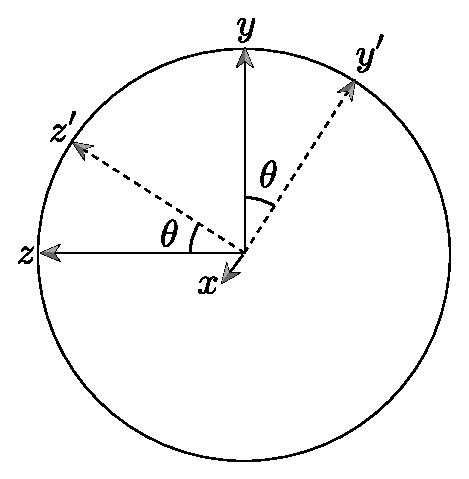
\includegraphics[scale=0.75]{chap02/Rotatexaxis.eps}
    \caption{绕$x$轴顺时针旋转角度$\theta$不改变$x$坐标。
        $y$和$z$轴映射为虚线给出的向量;$y$和$z$坐标相应变化。}
    \label{fig:2.11}
\end{figure}

容易看出矩阵不改变$x$轴:
\begin{align*}
    \bm R_x(\theta)[1\ 0\ 0\ 0]^\mathrm{T}=[1\ 0\ 0\ 0]^\mathrm{T}\, .
\end{align*}
它把$y$轴$(0,1,0)$映射为$(0,\cos\theta,\sin\theta)$,
把$z$轴映射为$(0,-\sin\theta,\cos\theta)$
\sidenote{译者注:这句话指的是旧坐标轴在新坐标系下的取值。}。
$y$和$z$轴仍在同一平面内,与$x$轴垂直,但旋转了给定角度。
空间中任意点也同样因该变换而绕$x$轴旋转并留在和之前同样的$yz$平面内。

函数\refvar{RotateX}{()}的实现很简单。
\begin{lstlisting}
`\refcode{Transform Method Definitions}{+=}\lastnext{TransformMethodDefinitions}`
`\refvar{Transform}{}` `\initvar{RotateX}{}`(`\refvar{Float}{}` theta) {
    `\refvar{Float}{}` sinTheta = std::sin(`\refvar{Radians}{}`(theta));
    `\refvar{Float}{}` cosTheta = std::cos(`\refvar{Radians}{}`(theta));
    `\refvar{Matrix4x4}{}` m(1,        0,         0, 0, 
                0, cosTheta, -sinTheta, 0,
                0, sinTheta,  cosTheta, 0,
                0,        0,         0, 1);
    return `\refvar{Transform}{}`(m, `\refvar[Matrix4x4::Transpose]{Transpose}{}`(m));
}
\end{lstlisting}

同样,绕$y$和$z$轴顺时针旋转,我们有
\begin{align*}
    \bm R_y(\theta)=\left[
        \begin{array}{cccc}
            \cos\theta  & 0 & \sin\theta & 0 \\
            0           & 1 & 0          & 0 \\
            -\sin\theta & 0 & \cos\theta & 0 \\
            0           & 0 & 0          & 1
        \end{array}
        \right], \quad
    \bm R_z(\theta)=\left[
        \begin{array}{cccc}
            \cos\theta & -\sin\theta & 0 & 0 \\
            \sin\theta & \cos\theta  & 0 & 0 \\
            0          & 0           & 1 & 0 \\
            0          & 0           & 0 & 1
        \end{array}
        \right]\, .
\end{align*}

{\ttfamily RotateY()}和{\ttfamily RotateZ()}的实现直接遵循上式此处不再介绍。

\subsection{绕任意轴旋转}\label{sub:绕任意轴旋转}
我们也提供了例程计算表示绕任意轴旋转的变换。
该通用矩阵的推导基于计算把给定轴映射为固定轴(例如$z$轴)的旋转,
执行旋转,再把固定轴旋转回原始轴。
更简洁的推导可以用向量代数构造
\sidenote{译者注:尽管下文的内容的图示和推导没太大问题,
    但想必读者第一次阅读时都会怀疑图中的标注和推导无法对应,
    以至于难以理解其含义。
    译者重新整理了这部分内容,详见\protect\refsub{四元数与旋转变换}。}。

考虑规范化的方向向量$\bm a$给出旋转轴,旋转角度为$\theta$,
被旋转向量为$\bm v$(\reffig{2.12})。
\begin{figure}[htbp]
    \centering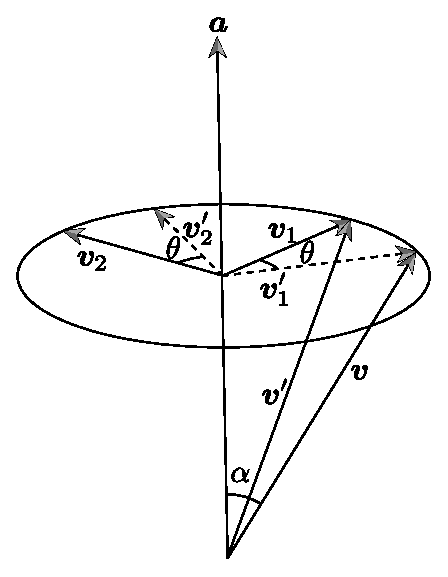
\includegraphics[scale=0.75]{chap02/Rotatearbitraryaxis.eps}
    \caption{向量$\bm v$可通过在垂直于任意轴$\bm a$且过$\bm v$末端的平面内
        建立坐标系统$(\bm p,\bm v_1,\bm v_2)$
        并绕$\bm p$旋转向量$\bm v_1$和$\bm v_2$来做到绕该轴旋转。
        将该旋转变换施加到坐标系统的轴$(1,0,0)$、$(0,1,0)$
        和$(0,0,1)$即给出该旋转的一般旋转矩阵。}
    \label{fig:2.12}
\end{figure}

首先,我们可以计算沿$\bm a$轴的向量$\bm v_\mathrm{c}$,
它在过$\bm v$的末端且平行于$\bm a$的平面内。
设$\bm v$和$\bm a$构成夹角$\alpha$,我们有
\begin{align*}
    \bm v_\mathrm{c}=\bm a\|\bm v\|\cos\alpha=\bm a(\bm v\cdot\bm a)\, .
\end{align*}

现在我们在该平面内计算一对基向量$\bm v_1$和$\bm v_2$。平凡地,其中一个是
\begin{align*}
    \bm v_1=\bm v-\bm v_\mathrm{c}\, ,
\end{align*}
且另一个可由叉积算得
\begin{align*}
    \bm v_2=(\bm v_1\times\bm a)\, .
\end{align*}

因为$\bm a$是规范化的,所以$\bm v_1$和$\bm v_2$长度相同,
都等于连接$\bm v$和$\bm v_\mathrm{c}$的向量的长度。
为了计算在旋转平面内绕$\bm v_\mathrm{c}$旋转角度$\theta$的变换,
之前的旋转公式已经给出
\begin{align*}
    \bm v'=\bm v_\mathrm{c}+\bm v_1\cos\theta+\bm v_2\sin\theta\, .
\end{align*}

为了将其转化为旋转矩阵,我们把该公式施加到
基向量$(1,0,0)$、$(0,1,0)$和$(0,0,1)$来得到矩阵各列的值。
以上所有结果封装在下列函数中。
如同其他旋转矩阵那样,其逆等于转置。
\begin{lstlisting}
`\refcode{Transform Method Definitions}{+=}\lastnext{TransformMethodDefinitions}`
`\refvar{Transform}{}` `\initvar{Rotate}{}`(`\refvar{Float}{}` theta, const `\refvar{Vector3f}{}` &axis) {
    `\refvar{Vector3f}{}` a = `\refvar{Normalize}{}`(axis);
    `\refvar{Float}{}` sinTheta = std::sin(`\refvar{Radians}{}`(theta));
    `\refvar{Float}{}` cosTheta = std::cos(`\refvar{Radians}{}`(theta));
    `\refvar{Matrix4x4}{}` m;
    `\refcode{Compute rotation of first basis vector}{}`
    `\refcode{Compute rotations of second and third basis vectors}{}`
    return `\refvar{Transform}{}`(m, `\refvar[Matrix4x4::Transpose]{Transpose}{}`(m));
}
\end{lstlisting}

\begin{lstlisting}
`\initcode{Compute rotation of first basis vector}{=}`
m.m[0][0] = a.x * a.x + (1 - a.x * a.x) * cosTheta;
m.m[0][1] = a.x * a.y * (1 - cosTheta) - a.z * sinTheta;
m.m[0][2] = a.x * a.z * (1 - cosTheta) + a.y * sinTheta;
m.m[0][3] = 0;
\end{lstlisting}

\begin{lstlisting}
`\initcode{Compute rotations of second and third basis vectors}{=}`
m.m[1][0] = a.x * a.y * (1 - cosTheta) + a.z * sinTheta;
m.m[1][1] = a.y * a.y + (1 - a.y * a.y) * cosTheta;
m.m[1][2] = a.y * a.z * (1 - cosTheta) - a.x * sinTheta;
m.m[1][3] = 0;

m.m[2][0] = a.x * a.z * (1 - cosTheta) - a.y * sinTheta;
m.m[2][1] = a.y * a.z * (1 - cosTheta) + a.x * sinTheta;
m.m[2][2] = a.z * a.z + (1 - a.z * a.z) * cosTheta;
m.m[2][3] = 0;
\end{lstlisting}

另外两个基向量的代码类似,此处不再介绍
\sidenote{译者注:笔者补充回来了。}。

\subsection{注视变换}\label{sub:注视变换}
\keyindex{注视变换}{look-at transformation}{transformation变换}对于
在场景中放置相机尤为有用。
调用者指定要求的相机位置、相机要注视的点以及
让沿这两个参数确定的观察方向的相机定向的“向上”向量。
所有这些值都用世界空间坐标给定。
然后注视的构建给出相机空间与世界空间之间的变换(\reffig{2.13})。
\begin{figure}[htbp]
    \centering%LaTeX with PSTricks extensions
%%Creator: Inkscape 1.0.1 (3bc2e813f5, 2020-09-07)
%%Please note this file requires PSTricks extensions
\psset{xunit=.5pt,yunit=.5pt,runit=.5pt}
\begin{pspicture}(173.80000305,146.08999634)
{
\newrgbcolor{curcolor}{0 0 0}
\pscustom[linewidth=1,linecolor=curcolor,linestyle=dashed,dash=4]
{
\newpath
\moveto(6.61000013,40.19999695)
\lineto(168.61000061,132.47999668)
}
}
{
\newrgbcolor{curcolor}{0 0 0}
\pscustom[linewidth=1,linecolor=curcolor]
{
\newpath
\moveto(5.5,137.98999596)
\lineto(5.5,39.30999756)
}
}
{
\newrgbcolor{curcolor}{0 0 0}
\pscustom[linestyle=none,fillstyle=solid,fillcolor=curcolor]
{
\newpath
\moveto(0,133.07999634)
\lineto(5.5,137.33999634)
\lineto(11.01,133.07999634)
\lineto(5.5,146.08999634)
\closepath
}
}
{
\newrgbcolor{curcolor}{0.65098041 0.65098041 0.65098041}
\pscustom[linestyle=none,fillstyle=solid,fillcolor=curcolor]
{
\newpath
\moveto(1.2,134.62999634)
\lineto(5.5,144.77999634)
\lineto(5.5,137.96999634)
\closepath
}
}
{
\newrgbcolor{curcolor}{0.40000001 0.40000001 0.40000001}
\pscustom[linestyle=none,fillstyle=solid,fillcolor=curcolor]
{
\newpath
\moveto(9.8,134.62999634)
\lineto(5.5,144.77999634)
\lineto(5.5,137.96999634)
\closepath
}
}
{
\newrgbcolor{curcolor}{0 0 0}
\pscustom[linewidth=1,linecolor=curcolor]
{
\newpath
\moveto(92.98999786,89.37999725)
\lineto(5.42000008,39.51999664)
}
}
{
\newrgbcolor{curcolor}{0 0 0}
\pscustom[linestyle=none,fillstyle=solid,fillcolor=curcolor]
{
\newpath
\moveto(86,91.73999634)
\lineto(92.42,89.05999634)
\lineto(91.45,82.16999634)
\lineto(100.03,93.38999634)
\closepath
}
}
{
\newrgbcolor{curcolor}{0.65098041 0.65098041 0.65098041}
\pscustom[linestyle=none,fillstyle=solid,fillcolor=curcolor]
{
\newpath
\moveto(87.95,91.45999634)
\lineto(98.89,92.73999634)
\lineto(92.97,89.36999634)
\closepath
}
}
{
\newrgbcolor{curcolor}{0.40000001 0.40000001 0.40000001}
\pscustom[linestyle=none,fillstyle=solid,fillcolor=curcolor]
{
\newpath
\moveto(92.2,83.98999634)
\lineto(98.89,92.73999634)
\lineto(92.97,89.36999634)
\closepath
}
}
{
\newrgbcolor{curcolor}{0 0 0}
\pscustom[linewidth=1,linecolor=curcolor]
{
\newpath
\moveto(106.23000336,3.52999878)
\lineto(5.5,39.54999542)
}
}
{
\newrgbcolor{curcolor}{0 0 0}
\pscustom[linestyle=none,fillstyle=solid,fillcolor=curcolor]
{
\newpath
\moveto(103.46,10.35999634)
\lineto(105.61,3.74999634)
\lineto(99.75,-0.00000366)
\lineto(113.86,0.79999634)
\closepath
}
}
{
\newrgbcolor{curcolor}{0.65098041 0.65098041 0.65098041}
\pscustom[linestyle=none,fillstyle=solid,fillcolor=curcolor]
{
\newpath
\moveto(104.52,8.70999634)
\lineto(112.62,1.23999634)
\lineto(106.21,3.52999634)
\closepath
}
}
{
\newrgbcolor{curcolor}{0.40000001 0.40000001 0.40000001}
\pscustom[linestyle=none,fillstyle=solid,fillcolor=curcolor]
{
\newpath
\moveto(101.62,0.60999634)
\lineto(112.62,1.23999634)
\lineto(106.21,3.52999634)
\closepath
}
}
{
\newrgbcolor{curcolor}{0 0 0}
\pscustom[linestyle=none,fillstyle=solid,fillcolor=curcolor]
{
\newpath
\moveto(173.80000162,131.3799963)
\curveto(173.80000162,136.92180968)(167.10020004,139.69615573)(163.18202122,135.77797691)
\curveto(159.2638424,131.85979809)(162.03818845,125.15999651)(167.58000183,125.15999651)
\curveto(173.12181521,125.15999651)(175.89616126,131.85979809)(171.97798244,135.77797691)
\curveto(168.05980362,139.69615573)(161.36000204,136.92180968)(161.36000204,131.3799963)
\curveto(161.36000204,125.83818292)(168.05980362,123.06383687)(171.97798244,126.98201569)
\curveto(175.89616126,130.90019451)(173.12181521,137.59999609)(167.58000183,137.59999609)
\curveto(162.03818845,137.59999609)(159.2638424,130.90019451)(163.18202122,126.98201569)
\curveto(167.10020004,123.06383687)(173.80000162,125.83818292)(173.80000162,131.3799963)
\closepath
}
}
\end{pspicture}

    \caption{给定相机位置、相机注视的位置以及一个“向上”方向,
        注视变换描述了来自左手观察坐标系统的变换,相机处于原点看向$+z$轴且$+y$轴向上。}
    \label{fig:2.13}
\end{figure}

为了求得注视变换矩阵的元素,
我们利用之前本节描述的原理:
变换矩阵的列给出了该变换作用于坐标系统基的结果。
\begin{lstlisting}
`\refcode{Transform Method Definitions}{+=}\lastnext{TransformMethodDefinitions}`
`\refvar{Transform}{}` `\initvar{LookAt}{}`(const `\refvar{Point3f}{}` &pos, const `\refvar{Point3f}{}` &look,
        const `\refvar{Vector3f}{}` &up) {
    `\refvar{Matrix4x4}{}` cameraToWorld;
    `\refcode{Initialize fourth column of viewing matrix}{}`
    `\refcode{Initialize first three columns of viewing matrix}{}`
    return `\refvar{Transform}{}`(`\refvar[Matrix4x4::Inverse]{Inverse}{}`(cameraToWorld), cameraToWorld);
}
\end{lstlisting}

最简单的是第四列,给出了相机空间原点$[0\ 0\ 0\ 1]^\mathrm{T}$映射到世界空间中的点。
显然它是用户提供的相机位置。
\begin{lstlisting}
`\initcode{Initialize fourth column of viewing matrix}{=}`
cameraToWorld.m[0][3] = pos.x;
cameraToWorld.m[1][3] = pos.y;
cameraToWorld.m[2][3] = pos.z;
cameraToWorld.m[3][3] = 1;
\end{lstlisting}

其他三列也不复杂。
首先\refvar{LookAt}{()}计算从相机位置到注视点的规范化方向向量;
这给出了$z$轴应该映射到的向量坐标,即矩阵第三列
(在左手坐标系统中,沿$+z$轴的观察方向定义相机空间)。
第一列给出相机空间中$+x$轴映射到世界空间的方向,
它通过取用户提供的“向上”向量与刚刚计算的观察方向向量的叉积求得。
最后,“向上”向量通过重新计算观察方向向量与变换的$x$轴向量的叉积求得,
这样保证了$y$和$x$轴是垂直的,并且我们获得了一个正交观察坐标系统。
\begin{lstlisting}
`\initcode{Initialize first three columns of viewing matrix}{=}`
`\refvar{Vector3f}{}` dir = `\refvar{Normalize}{}`(look - pos);
`\refvar{Vector3f}{}` right = `\refvar{Normalize}{}`(`\refvar{Cross}{}`(`\refvar{Normalize}{}`(up), dir));
`\refvar{Vector3f}{}` newUp = `\refvar{Cross}{}`(dir, right);
cameraToWorld.m[0][0] = right.x;
cameraToWorld.m[1][0] = right.y;
cameraToWorld.m[2][0] = right.z;
cameraToWorld.m[3][0] = 0.;
cameraToWorld.m[0][1] = newUp.x;
cameraToWorld.m[1][1] = newUp.y;
cameraToWorld.m[2][1] = newUp.z;
cameraToWorld.m[3][1] = 0.;
cameraToWorld.m[0][2] = dir.x;
cameraToWorld.m[1][2] = dir.y;
cameraToWorld.m[2][2] = dir.z;
cameraToWorld.m[3][2] = 0.;
\end{lstlisting}